\clearpage\section {Линеен едносвързан и двусвързан списък}

\subsection {Представяне на двусвързан списък}

\begin{mdframed}[hidealllines=true,backgroundcolor=gray!20]
Възел на линеен двусвързан списък представяме със следния шаблон на структура:
\begin{verbatim}
template <class T>
struct dllnode
{
  T data;
  dllnode<T> *next, *previous;
};
\end{verbatim}
Освен ако не е указано друго, задачите по-долу да се решат като се реализират методи на клас \code{DLList} със следния скелет:
\begin{verbatim}
template <class T>
class DLList
{
  //...
  private:
  dllnode<T> *first, *last;
};
\end{verbatim}
Преди да пристъпите към задачите, реализирайте подходящи контруктори, деструктор и оператор за присвояване на класа.
\end{mdframed}

\begin{figure}
    \centering
  
      \begin{tikzpicture}[auto, node distance=2cm,>=latex']
      \node[lnode] (n1) {\nodepart{two}1};
      \node[lnode, right of = n1] (n2) {\nodepart{two}2};
      \node[lnode, right of = n2] (n3) {\nodepart{two}3};
      \node[lnode, right of = n3] (n4) {\nodepart{two}4};
      \node[lnode, right of = n4] (n5) {\nodepart{two}5};
  
      \node[rectangle,left of = n1](start){};
  
      \draw[*->]  (start)-- (n1);
  
      \draw[*->] let \p1 = (n2.three), \p2 = (n1.center) in (\x1,\y2) -- (n3);
      \draw[*->] let \p1 = (n1.three), \p2 = (n1.center) in (\x1,\y2) -- (n2);
      \draw[*->] let \p1 = (n3.three), \p2 = (n1.center) in (\x1,\y2) -- (n4);
      \draw[*->] let \p1 = (n4.three), \p2 = (n1.center) in (\x1,\y2) -- (n5);
      \draw[*->,dashed] let \p1 = (n2.one), \p2 = (n1.center) in ([shift={(0.1cm,-0.1cm)}]\x1,\y2) |-([shift={(0,0.5cm)}]n2.north west) -- ([shift={(0,0.5cm)}]n1.north) -| ([shift={(-1cm,0cm)}]n1);
      \draw[*->,dashed] let \p1 = (n3.one), \p2 = (n2.center) in ([shift={(0.1cm,0.1cm)}]\x1,\y2) |-([shift={(0,-1cm)}]n3.north west) -- ([shift={(0,-1cm)}]n2.north) -| ([shift={(-1cm,0cm)}]n2);
      \draw[*->,dashed] let \p1 = (n4.one), \p2 = (n3.center) in ([shift={(0.1cm,-0.1cm)}]\x1,\y2) |-([shift={(0,0.5cm)}]n4.north west) -- ([shift={(0,0.5cm)}]n3.north) -| ([shift={(-1cm,0cm)}]n3);
      \draw[*->,dashed] let \p1 = (n5.one), \p2 = (n4.center) in ([shift={(0.1cm,0.1cm)}]\x1,\y2) |-([shift={(0,-1cm)}]n5.north west) -- ([shift={(0,-1cm)}]n4.north) -| ([shift={(-1cm,0cm)}]n4);
      \end{tikzpicture}
    \caption{Двусвързан списък}
    \label{fig:skiplist}
  \end{figure}
  

Следните задачи да се решат като упражнение за директно боравене с възлите на линеен двусвързан списък. Функциите (методите) да се тестват с подходящи тестове.

\begin{enumerate}

	\item  Да се дефинира функция \code{int count(dllnode<T>* l,int x)}, която преброява колко пъти елементът \code{x} се среща в списъка с първи елемент \code{l}.
	\item  Фунцкция \code{dllnode<int>* range (int x, int y)} която създава и връща първия елемент на списък с елементи $x, x+1, ..., y$, при положение, че $x \leq y$.
	\item  Да се дефинира функция \code{removeAll (dllnode<T>*\& l,const T\& x)}, която изтрива всички срещания на елемента \code{x} от списъка \code{l}.
	\item  Да се дефинира функция \code{void append(dllnode*<T>\& l1, dllnode<T>* l2)}, която добавя към края на списъка $l_1$ всички елементи на списъка $l_2$. Да се реализира съответен оператор \texttt{+=} в класа на списъка.
	\item  Да се дефинира функция \code{dllnode* concat(dllnode<T>* l1, dllnode<T>* l2)}, който съединява два списъка в нов, трети списък. Т.е. \code{concat($l_1,l_2$)} създава и връща нов списък от елементите на \code{$l_1$}, следвани от елементите на \code{$l_2$}. Да се реализира съответен оператор \texttt{+} в класа на списъка.
	\item  Да се дефинира функция \code{reverse}, която обръща реда на елементите на списък. Например, списъкът с елементи $1,2,3$ ще се преобразува до списъка с елементи $3,2,1$.
	\item Да се напише функция \code{void removeduplicates (dllnode *\&l)}, която изтрива всички дублиращи се елементи от списъка $l$.
  \item За шаблона \texttt{DLList} да се реалзиира изтриване на елемент по индекс.
\end{enumerate}

\subsection {Списъци и сложности}
\label{timing}
\begin{mdframed}[hidealllines=true,backgroundcolor=gray!20]
Функцията \code{std::clock()} от \code{<ctime>} връща в абстрактни единици времето, което е изминало от началото на изпълнение на програмата. Обикновено тази единица за време, наречена ``\code{tick}'', е фиксиран интервал ``реално'' време, който зависи от хардуера на системата и конфирграцията ѝ. Константата \code{CLOCKS\_PER\_SEC} дава броя \code{tick}-ове, които се съдържат в една секунда реално време.

Чрез следния примерен код може да се измери в милисекунди времето за изпълнение на програмния блок, обозначен с ``...''.
\begin{verbatim}
clock_t start = std::clock();
//...
clock_t end = std::clock();

long milliseconds = (double)(end-start)/
                    (CLOCKS_PER_SEC/1000.0);

\end{verbatim}
\end{mdframed}

\begin{enumerate}[resume]

\item За шаблона DLList да се дефинира метод \texttt{size\_t find(const T\& x)}, който намира поредния номер на елемента \texttt{x} в списъка (или връща размера на списъка, ако такъв елемент няма). Да се напише подходящ тест и да се изследва времевата сложност на метода емпирично.

\item Да се изпробват поне две различни стратегии за разширяване на динамичен масив (например, увеличаване на размера с 1 и с коефициент). Да напишат подходящи тестове и да се сравнят производителностите на двата подхода емпирично.

\end{enumerate}


\subsection{SList (опростен вариант на Skip List)}

\begin{mdframed}[hidealllines=true,backgroundcolor=gray!20]
Разглеждаме \emph{опростена} реализация на структурата от данни Skip List (``Списък с прескачене, СП''). Възелът на линейния едносвързан списък разширяваме с още един указател към следващ елемент:

\begin{verbatim}
template <class T>
struct lnode
{
  T data;
  lnode<T> *next, *skip;
};
\end{verbatim}
Както и при стандартния едносвързан списък, всеки от елментите на СП съдържа в указателя \code{next} адреса на непосредствения си съсед. Елементите на списъка са под дадена наредба. Някои от елементите могат да съдържат в указателя \code{skip} дреса на друг елемент, намиращ се по-напред в редицата от елементи (вж. Фигура \ref{fig:skiplist}). Например, нека имаме СП с $n$ елемента в нарастващ ред. Ако списъкът е построен така, че всеки $\sqrt{n}$-ти елемент има указател към следващия  $\sqrt{n}$-ти елемент, то търсенето на подсписъка, съдържащ даден елемент, ще бъде със сложност $O(\sqrt{n})$. Търсенето в рамките на подсписъка с $\sqrt{n}$ елемента остава линейно. Идеята може да се продължи така, че всеки елемент да може да има и по-голям брой указатели към елементи все по-напред в СП, но за нашите цели ще се ограничим до описания прост СП.

Следващите задачи изискват реализация на клас \code{SList} с основните му канонични методи и метод за построяване на ``бързите връзки''. Реализирайте обиновен метод за вмъкване на елементи \code{insertSorted}, който вмъква елементи грижейки се само за непосредствените връзки (\code{next}), и метод \code{speedup}, който построява бързите връзки в списъка, след като в него са вмъкнати определен брой елементи.
\end{mdframed}

\begin{figure}
  \centering

    \begin{tikzpicture}[auto, node distance=2cm,>=latex']
    \node[lnode] (n1) {\nodepart{two}1};
    \node[lnode, right of = n1] (n2) {\nodepart{two}2};
    \node[lnode, right of = n2] (n3) {\nodepart{two}3};
    \node[lnode, right of = n3] (n4) {\nodepart{two}4};
    \node[lnode, right of = n4] (n5) {\nodepart{two}5};

    \node[rectangle,left of = n1](start){};

    \draw[*->]  (start)-- (n1);

    \draw[*->] let \p1 = (n2.three), \p2 = (n1.center) in (\x1,\y2) -- (n3);
    \draw[*->] let \p1 = (n1.three), \p2 = (n1.center) in (\x1,\y2) -- (n2);
    \draw[*->] let \p1 = (n3.three), \p2 = (n1.center) in (\x1,\y2) -- (n4);
    \draw[*->] let \p1 = (n4.three), \p2 = (n1.center) in (\x1,\y2) -- (n5);
    \draw[*->,dashed] let \p1 = (n1.one), \p2 = (n1.center) in ([shift={(0.1cm,-0.1cm)}]\x1,\y2) |-([shift={(0,0.5cm)}]n1.north east) -- ([shift={(0,0.5cm)}]n3.north) -| (n3);
    \draw[*->,dashed] let \p1 = (n3.one), \p2 = (n3.center) in ([shift={(0.1cm,0.1cm)}]\x1,\y2) |-([shift={(0,-0.5cm)}]n3.south east) -- ([shift={(0,-0.5cm)}]n5.south) -| (n5);
    \end{tikzpicture}
  \caption{Списък с прескачане}
  \label{fig:skiplist}
\end{figure}

\begin{enumerate}[resume]


  \item  Да се реализират конструктор за копиране и оператор на присвояване на \code{SList}, които репликират и бързите връзки.
  \item Да се подобри методът за вмъкване на елемент \code{insertSorted}. Ако при вмъкване на нов елемент някой подсписък (обособен от дадена бърза вързка) получи повече от $2\sqrt(n)$ елемента, да се добави нова бърза връзка така, че подсписъка да се раздели на два подсписъка.
	\item  Да се извърши времево измерване на проблема за търсене на елемент в подреден \code{SList}, както е обяснено в Секция \ref{timing}, и да се изобрази чрез графика. Да се извършат емпирични сравнения на производителността на търсенете със и без оптимизацията.

\end{enumerate}


\pagebreak

\subsection {Итератори за линейни СД}
\label{iterators1}
Следните задачи да се решат като упражнение за работа с итератори. Задачите изискват реализация на клас линеен двусвързан списък и \code{forward} итератор за него. Всяка функциия да се тества с подходящи тестове.


\begin{enumerate}[resume]

	\item Да се разшири интераторът на двусвързан списък така, че да поддържа оператора за стъпка назад \texttt{-{}-}.

	\item Да се напише функция \code{bool duplicates (...)}, която проверява дали в контейнер има дублиращи се елементи.

	\item Да се напише фунцкия \code{bool issorted (...)}, която проверява дали елементите на даден контейнер са подредени в нарастващ или в намаляващ ред.

	\item Да се напише фунцкия \code{bool palindrom (...)}, която проверява дали редицата от елементите на даден контейнер обрзува палиндром (т.е. дали се чете еднакво както отляво надясно така и отдяно наляво).

	\item Да се реализира константен итератор за двусвързани списъци и горните функции да се преработят така, че да могат да работят с константни итератори.

    

\end{enumerate}

\subsection {Функции от високо ниво и оператори над итератори}

\begin{mdframed}[hidealllines=true,backgroundcolor=gray!20]
  Нека ``поредица'' да наричаме последователни елементи на някакъв контейнер, зададени чрез итератори към началото и края на последователността. С помощта на следния шаблон:
  \begin{verbatim}
template <class Iterator>
class Sequence{
    public:
        Sequence (const Iterator &b, 
                  const Iterator &e):_begin(b), _end (e){}
        Iterator begin()
        {return _begin;}
        Iterator end()
        {return _end;}
    private:
        Iterator _begin;
        Iterator _end;
};
  \end{verbatim}

  става възможно не само да оформим двойката начало-край в общ обект, но и да итерираме съответната поредица с цикъл \code{for}. Ако \code{begin} и \code{end} са съответните итератори към елементи от тип \code{E} и имаме обекта \code{Sequence<SomeIterator>(begin,end)}, то можем да направим обхождането:
 \begin{verbatim}
for (E& x : seq){...}   
 \end{verbatim}
 
 На лекции разглеждаме деструктивен вариант на функцията от високо ниво \code{map}, извършваща еднотипна трансформация на елементите на поредица, като се абстрахира напълно от контейнера:
  
\begin{verbatim}
template <class Iterator, class Element>
void map(Sequence<Iterator> seq,
          Element (*f)(const Element &))
{
    for (Element& e: seq)
    {e = f (e);}    
}
\end{verbatim}

  Може да разгледаме и фунцкията за агрегации \code{reduce}, позната от функционалното програмиране: 
\begin{verbatim}
template <class Iterator, class Element>
Element reduce(Sequence<Iterator> seq,
                Element (*op)(const Element &, const Element &),
                Element null_val)
{
    Element accum = null_val;
    for (Element e : seq)
    { accum = op(accum, e); }
    return accum;
}
\end{verbatim}
Възможно е също да реализираме операция с поредица, която изменя броя или реда на елементите ѝ, отново без знание за подлежащия контейнер. Такава е например операцията \code{filter}. Това налага да се конструира нова поредица, като по някакъв начин се измени поведението на итераторите на оригиналната поредица. Например, реализирания на лекции \code{FilterIterator} ``изменя'' даден друг итератор като ``прескача'' елементите, които не удовлетворяват даден предикат. По този начин можем да дефинираме:
\begin{verbatim}
template <class Iterator, class Element>
Sequence<FilterIterator<Iterator,Element>> 
    filter(Sequence<Iterator> &seq,
           bool (*pred)(const Element &))
{
  FilterIterator<Iterator,Element> begin (seq.begin(),seq.end(),pred);
  FilterIterator<Iterator,Element> end (seq.end(),seq.end(),pred);

  return Sequence<FilterIterator<Iterator, Element>> (begin, end);
}    
  \end{verbatim}
  Използването на \code{Sequence} както за параметър, така и за резултат на тези функции, ни позволява да ги използваме за обхождане на новополучените подредици. Също така, можем да композираме функциите:
  \begin{verbatim}
for (E x : filter (seq, even)) {...обработка само на четните елементи на seq...}
reduce(filter(seq,even),plus,0);//сума на четните елементи на seq 
  \end{verbatim}
Ако по подобие на \code{FilterIterator} реализираме \code{MapIterator}, можем да напраивм функционален вариант на \code{map}, \code{mapf}. Това ще ни позволи на намерим сумата на четните елементи на поредица, след като ги увеличим с единица, по следния начин:
\begin{verbatim}
reduce(mapf(filter(seq,even), inc), plus, 0)  
\end{verbatim}
\end{mdframed}

\begin{enumerate}[resume]
  \item По аналогия на дадените примери да се дефинира функция \code{append(a,b)}, която създава нова поредица чрез слепване на поредиците \code{a} и \code{b}.
  \item По аналогия на дадените примери да се дефинира функция \code{combine(a,b,f)}, която създава нова поредица от стойностите на двуместната функция \code{f}, приложена върху съответните елементи на \code{a} и \code{b}. Функцията да се демомстрира като се съберат съответните елементи на две редици.
  \item По аналогия на дадените примери да се дефинира функция \code{merge(a,b)}. Ако $a=a_1,...,a_k$, $b=b_1,...,b_l$, то $merge(a,b)=a_1,b_1,a_2,b_2,...$. 
  \item По аналогия на дадените примери да се дефинира функция \code{zip(a,b)}, която създава нова поредица от двойките (\code{std::pair}) от стойностите на съответните елементи на \code{a} и \code{b}. 
\end{enumerate}


\section {Приложения на структурата от данни стек}

\subsection {Общи задачи за стекове}

\begin{enumerate}
  \item Нека е даден масив с $n$ елемента. За всеки от елементите на масива да се изведе следващия в масива по-голям елемент. Т.е. за всеки елемент $a[i]$ да се отпечата $a[j]$ такъв, че $n>j>i$ и $\forall k \in (i,j):a[k] \leq a[i]$. Ако такъв елемент няма, да се изведе числото $-1$. Пример, за масива \verb#{4, 5, 2, 25}#, да се изведат двойките \verb#(4,5), (5,25), (2,25), (25,-1)#. Алгоритъмът да работи с линейна сложност спрямо $n$. \emph{Упътване: Задачата е известна под името ``Next Greater Element(NGE)''}.
\end{enumerate}

\subsection {Изрази и стекове}

\begin{enumerate}[resume]
  \item Даден е израз, който може да съдържа отварящи и затварящи скоби.  Да се напише функция, която проверява дали скобите на израза са  правилно балансирани. Например, изразът \code{(x+(y+(1+2)))} считаме за правилно балансиран, но не и израза \code{(x+y)*3)+(x+(1+2)}.
  \item Да се реши горната задача при положение, че изразът може да има едновременно кръгли, фигурни и квадратни скоби.

\end{enumerate}


\begin{mdframed}[hidealllines=true,backgroundcolor=gray!20]
  По време лекции разглеждаме реализация на \emph{Shunting Yard} алгоритъма за пребразуване на инфиксен аритметичен израз в постфиксен вид (Обратен полски запис). Реализацията работи само с двуместни оператори и скоби, като отчита приоритет на операциите.
\end{mdframed}

\begin{enumerate}[resume]
  \item При изчисляването на стойността на постфиксен израз, да се разгледа случая на ляво-асоциативни оператори (като деление и изваждане).
  \item При изчисляването на стойността на постфиксен израз, да се позволи използването на едноместни функции без влагане. Да се поддържа ограничен набор от предефинирани функции (напр. $sin(x)$ и $\sqrt{x}$.). Функциите да са само едноместни и да не се позволява влагане на извиквания.
  \item Да се преработи алгоритъма за изчисляването на стойността на постфиксен израз така, че да се генерира прав полски запис (префиксна нотация).
\end{enumerate}

\subsection {Цикъл със стек вместо рекурсия}

\underline{Упътване}:Решете задачите с рекурсия и след това преобразувайте решението в решение със стек.


\begin{enumerate}[resume]

 \item (*)Да се дефинира функция за намиране на стойността на полинома на Ермит $Hn(x)$ (x е реална променлива, а n неотрицателна цяла променлива), дефиниран по следния начин:

 $H_0(x)=1$

 $H_1(x)=2x$

 $H_n(x)=2xH_{n-1}(x)+2(n-1)H_{n-2}(x), n>1$,

 за дадени $n$ и $x$ \underline{с използване на стек}.


 \item Нека е дадена абстрактна шахматна дъска с размери $n \times n$, $4 \le n \le 8$ и число $k$, $0 \le k \le n$. Казваме, че разположени на дъската  $k$ коня образуват ``валидна конфигурация'', ако никоя фигура не е поставена на поле, което се ``бие'' от друга фигура според съответните шахматни правила.

 Да се дефинира клас \texttt{KnightConfig}, представящ ``конфигуратор'' на шахматни коне. Конструкторът на класа инициализира конфигуратора с числата $n$ и $k$. Класът позволява ``обхождането'' една по една на всички валидни конфигурации за дадените параметри, по подобие на \texttt{forward} итератор на структура от данни. Класът да притежава следните методи:

 \begin{itemize}
   \item \texttt{void KnightConfig::printCurrentConfig()}: Отпечатва текущо намерената конфигурация.
     Пример за отпечатана конфигурация с $n=5, k=2$:
     \begin{verbatim}
     _ _ _ _ _
     _ _ H _ _
     _ _ _ _ _
     _ _ _ _ H
     _ _ _ _ _

     \end{verbatim}
   \item \texttt{void KnightConfig::findNextConfig()}: Намира следваща конфигурация.
   \item \texttt{bool KnightConfig::noMoreConfigs()}: Показва дали всички възможни конфигурации са вече изчерпани.
 \end{itemize}

 \item Да се реши задачата за Ханойските кули с използване на стек.

 Да се дефинира клас \texttt{HanoyPlayer} със следните методи:

 \begin{itemize}
   \item Конструктор с параметър, указващ броя дискове върху лявото колче за началното състояние на играта.
   \item Метод \texttt{bool final()}, който показва дали играта е достигнала финанлно състояние (т.е. всички дискове са на дясното колче).
   \item Метод \texttt{makeMove()}, който извършва един ход от играта.
   \item Метод \texttt{printBoard()}, който отпечатва текущото състояние на игровата дъска, например по следния начин:
     \begin{verbatim}

        2
        3     1
        5  *  4
     \end{verbatim}
   На примера е изобразено състояние на играта, при което на лявото колче има три диска - с размери 5, 3 и 2, на средното колче няма дискове, а на дясното има два диска - с размери 4 и 1.

 \end{itemize}

\end{enumerate}

\pagebreak

\section {Двоични дървета}

\subsection {Прости обхождания}

\begin{mdframed}[hidealllines=true,backgroundcolor=gray!20]
Възел на двоично дърво представяме със следния шаблон на структура:
\begin{verbatim}
template <class T>
struct BinTreeNode
{
  T data;
  BinTreeNode *left, *right;
  //... помощни конструктори
};
\end{verbatim}
Освен ако не е указано друго, задачите по-долу да се решат като се реализират методи на клас \code{BinTree} със следния скелет:
\begin{verbatim}
template <class T>
class BinTree
{
  //...
  private:
  BinTreeNode<T> *root;
};
\end{verbatim}
\end{mdframed}

\begin{enumerate}[]

	\item Да се деифнира метод \texttt{count} на клас \texttt{BinTree}, който намира броя на елементите на дървото.

	\item Да се деифнира метод \texttt{countEvens} на клас \texttt{BinTree}, който намира броя на елементите на дърво от числа, които са четни.


	\item Да се дефинира метод \texttt{int BTree<T>::searchCount (bool (*pred)(const T\&))} към клас \texttt{BinTree}, който намира броя на елементите на дървото, които удовлетворяват предиката \texttt{pred}.

	Да се приложи \texttt{searchCount} за решаване на горните две задачи.

	\item Да се дефинира метод \texttt{bool BinTree<T>::height ()}, намиращ височината на дърво. \textit{Височина на дърво наричаме дължината (в брой върхове) на най-дългия път от корена до кое да е листо на дървото.}
	\textit{Пример. Височината на дървото на Фигура \ref{fig:tree1} е \textbf{3}.}

  \begin{figure}
  \centering
	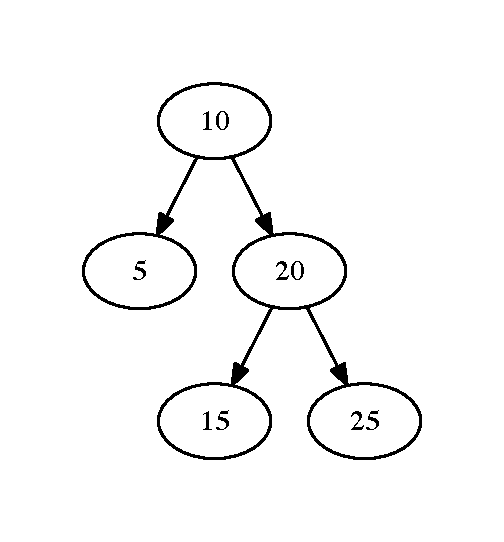
\includegraphics[width=4cm]{images/tree1}

	\caption{Двоично наредено дърво}
  \label{fig:tree1}
  \end{figure}


	\item Да се деифнира метод \texttt{countLeaves} на клас \texttt{BinTree}, който намира броя на листата в дървото.

	\item Да се деифнира метод \texttt{maxLeaf} на клас \texttt{BinTree}, който намира най-голямото по стойност листо на непразно дърво. Да се приеме, че за типа \texttt{T} на шаблона \texttt{BinTree} е дефиниран операторът \texttt{<}.

	\item Нека е дадено дървото \texttt{t} и низът \texttt{s}, съставен само от символите `L' и `R' ($s \in \{L,R\}^*$). Нека дефинираме ``съответен елемент'' на низа \texttt{s} в дървото \texttt{t} по следния начин:
	\begin{itemize}
		\item Ако дървото \texttt{t} е празно, низът \texttt{s} няма съответен елемент
		\item Ако низът \texttt{s} е празен, а дървото \texttt{t} - не, то коренът на дървото \texttt{t} е съответният елемент на низа \texttt{s}
		\item Ако първият символ на низа \texttt{s} е `L' и дървото \texttt{t} не е празно, то съответният елемент на низа \texttt{s} в дървото \texttt{t} е съответният елемент на низа $s+1$ в \textbf{лявото} поддърво на \texttt{t}
		\item Ако първият символ на низа \texttt{s} е `R' и дървото \texttt{t} не е празно, то съответният елемент на низа \texttt{s} в дървото \texttt{t} е съответният елемент на низа $s+1$ в \textbf{дясното} поддърво на \texttt{t}
	\end{itemize}

	\textit{Пример. За 	дървото от Фигура \ref{fig:tree1}, съответният елемент на празния низ е 10, на низа ``RL'' е 15, а ``RLR'' няма съответен елемент.}

	Да се дефинира метод \texttt{T\& BinTree<T>::getElement (const char *s)}, който намира съответния елемент на низа \texttt{s}. Какво връща методът в случаите на липса на съответен елемент е без значение.


\end{enumerate}

\subsection {Отпечатване и сериализация}

\begin{mdframed}[hidealllines=true,backgroundcolor=gray!20]
  В следващите задачи се очаква дефинирането на външни за класа на дървото функции, вместо методи на класа, както в уводните задачи. За целта се използва клас \code{Position}, заместващ указател към възел в дадено дърво, по подобие на итератор, и с чиято помощ може да се извърши рекурсивно обхождане на дървото.
  \begin{verbatim}
template <class T>
class Position 
{
public:
    Position<T> left () const;
    Position<T> right () const;
    T operator * () const;
    bool empty () const;
    //...
};
  \end{verbatim}

  В условията по-долу с \code{[подходящ тип]} е указано, че част от задачата е да се изберат правилните типове на параметрите на фунцкиите така, че рекурсия да може да се осъществи.
\end{mdframed}
  
\begin{enumerate}[resume]

  \item Да се дефинира функция \texttt{prettyPrint ([подходящ тип]t)}, отпечатваща двоично дърво на стандарния изход по следния начин: (1) всеки наследник е вдясно от родителя си, (2) елементите на еднакво ниво в дървото се отпечатват на еднаква колона от екрана, (3) десните наследници са на предишен ред от родителя си и (4) левите наследни са следващ ред спрямо родителя си.

  Например, дървото от Фигура \ref{fig:tree1} би изглеждало по следния начин (да се отпечатат и номерата на редовете на стандартния изход):

  \begin{verbatim}
  1:        25
  2:    20
  3:        15
  4: 10
  5:    5
  \end{verbatim}



  \item Да се дефинират функции \code{std::string serializeTree ([подходящ тип]t)} и \code{BinTree<int> parseTree (std::string)} за сериализация и де-сериализация на двоично дърво, съдържащо числа, като се използва ``\texttt{Scheme} формат''.
  
   Може ли да се сериализира дърво, съдържащо други дървета?
\end{enumerate}

\begin{mdframed}[hidealllines=true,backgroundcolor=gray!20]
Представяне на двоично дърво в ``Scheme формат'' наричаме еднозначно текстово представяне на структурата от данни, образувано по следните правила:
\begin{itemize}
  \item Празното дърво се прдставя с низа ``()''
  \item Нека е дадено дървото $t$ с корен $x$, ляво поддърво $t_l$ и дясно поддърво $t_r$. Ако $s_l$ е представянето в ``Scheme формат'' формат на $t_l$, а $s_r$ е представянето в ``Scheme формат'' на $t_r$, то низът ``($x$ $s_l$ $s_r$)'' е представянето на дървото $t$, кдето ``$x$'', ``$s_l$'' и ``$s_r$'' са съответните низове.

\end{itemize}
Например, дървото от Фигура \ref{fig:tree1} се представя по следния начин:

\begin{verbatim}
(10 (20 (25 () ()) (15 () ())) (5 () ()))
\end{verbatim}

\end{mdframed}

\subsection {Обхождания}
\begin{enumerate}[resume]

  \item Да се реализира функция \texttt{std::vector<T> listLeaves ([подходящ тип]t)} намираща списък със стойностите на листата на дървото.

  \item Да се дефинира функция \texttt{std::string findTrace ([подходящ тип]t, const T\& x)}. Ако \texttt{x} е елемент на дървото, функцията да връща следата на \texttt{x} (според дефиницията на ``следа'', обсъдена на лекции). Ако \texttt{x} не е елемент на дървото, функцията да връща низа ``\_''.

  \textit{Пример: За дървото от Фигура \ref{fig:tree1}, следата на елемента със стойност 25 е ``RR''}.
    
  \item Да се дефинира функция \texttt{T getAt([подходящ тип]t, size\_t i)}, която намира $i$-тият пореден елемент на дървото при обхождане корен-ляво-дясно.
  
  Пример: За дървото от Фигура \ref{fig:tree1}, елементът с пореден номер 0 е 10, с номер 1 е 5, с номер 2 е 20 и т.н.
  
\end{enumerate}

\subsection {Представяне на аритметичен израз чрез дърво}
\begin{enumerate}[resume]
\item Нека е даден израз, построен по правилата на следната граматика:

\begin{verbatim}
<expression> ::= <digit> | (<expression><operator><expresson>)
<digit> ::= 1..9
<operator> ::= + | - | * | /
\end{verbatim}

Да се реалзира функция на клас \code{BinTree<char> parseExpression (std::string s)}, която по правилно построен израз, записан в низа \texttt{s}, създава двоично дърво от символи, представящо израза по следното правило:
\begin{itemize}
  \item Ако изразът е от типа ``\texttt{x}'', където \texttt{x} е цифра, то съответното му дърво е листо със стойност символа \texttt{x}.
  \item Ако изразът е от типа ``\texttt{(<израз 1><op><израз 2>)}'', то съответното му дърво има като стойност на корена символа на съответния оператор, ляво поддърво, съответно на \texttt{<израз 1>} и дясно поддърво, съответно на \texttt{<израз 2>}.
\end{itemize}

Дървото на Фигура \ref{fig:treeexpr} съответства на изарза \code{(1*(2+3))}.

\begin{figure}
\centering
\begin{tikzpicture}[auto, node distance=2cm,>=latex']
\node [treenode] {*}
  child {
    node [treenode] {1}
  }
  child {
    node [treenode] {+}
    child {
      node [treenode] {2}
    }
    child {
      node [treenode] {3}
    }
  };
\end{tikzpicture}
\caption{Дърво на израза \code{(1*(2+3))}.}
\label{fig:treeexpr}
\end{figure}

\item Да се реализира функция \texttt{double calculateExpresisonTree ([подходящ тип]t)}, която намира стойността на израз по дадено дърво, построено от решението на предишната задача.

\end{enumerate}

\subsection {Построяване и модификации на дърво}

\begin{enumerate}[resume]

  \item По дадено число $h$ да се построи идеално балансирано двоично дърво с височина $h$. Стойността на всеки от елементите на дървото да е равна на нивото, в което се намира елемента (вж. Фигура \ref{fig:balanced}).

  \begin{figure}
  \centering
  \begin{tikzpicture}[auto, sibling distance=5cm,>=latex',level 2/.style={sibling distance=3cm}]
  \node [] {0}
    child {
      node [] {1}
        child {
          node []{2}
        }
        child {
          node []{2}
        }
    }
    child {
      node [] {1}
      child {
        node []{2}
      }
      child {
        node []{2}
      }
    };
  \end{tikzpicture}
  \caption{Идеално балансирано двоично дърво с височина 3}
  \label{fig:balanced}
  \end{figure}

  \item {Нека е даден символен низ $s$ с дължина $n$. Нека $h$ е такова, че $2^h \geq n > 2^{h-1}$ } (минималната височина на двоично дърво, което има поне $n$ листа в последното си ниво). Да се дифинира функция, която по даден низ $s$ построява двоично дърво от символи с височина $h$, такова, че низът $s$ е разположен в листата на дървото, четени от ляво надясно. Възлите на дървото, които не са листа, да съдържат символа интервал. Вж. Фигура \ref{fig:stringleaves}

  \begin{figure}
  \centering
  \relscale{0.75}
  \begin{tikzpicture}[auto, sibling distance=8cm,>=latex',level 3/.style={sibling distance=5cm},level 2/.style={sibling distance=4cm},level 3/.style={sibling distance=2cm}]
  \node [treenode] {}
    child {
      node [treenode] {}
        child {
          node [treenode]{}
          child {
            node [treenode]{H}
          }
          child {
            node [treenode]{e}
          }
        }
        child {
          node [treenode]{}
          child {
            node [treenode]{l}
          }
          child {
            node[treenode] {l}
          }
        }
    }
    child {
      node [treenode] {}
      child {
        node [treenode]{}
        child {
          node [treenode]{o}
        }
        child {
          node [treenode]{!}
        }
      }
      child [missing]
    };
  \end{tikzpicture}
  \caption{Дърво, в чиито листа е разположен низът ``Hello!''}
  \label{fig:stringleaves}
  \end{figure}


  \item Стойността на всеки възел \texttt{V} в дадено двоично дърво от числа да се замени с броя на всички елементи на поддървото, на което \texttt{V} е корен. Вж. Фигура \ref{fig:treenodecount}. 
  
  \emph{При операцията всеки от възлите да бъде посетен най-много веднъж!}

  \begin{figure}
  \centering
  \begin{tabular}{c c}
  \begin{tikzpicture}[auto, node distance=2cm,>=latex']
  \node [treenode] {10}
    child {
      node [treenode] {5}
      child {
        node [treenode] {2}
      }
      child [missing]
    }
    child {
      node [treenode] {20}
      child {
        node [treenode] {15}
      }
      child {
        node [treenode] {25}
        child {
          node [treenode] {22}
        }
        child [missing]
      }
    };
  \end{tikzpicture}
   &
   \begin{tikzpicture}[auto, node distance=2cm,>=latex']
   \node [treenode] {7}
     child {
       node [treenode] {2}
       child {
         node [treenode] {1}
       }
       child [missing]
     }
     child {
       node [treenode] {4}
       child {
         node [treenode] {1}
       }
       child {
         node [treenode] {2}
         child {
           node [treenode] {1}
         }
         child [missing]
       }
     };
   \end{tikzpicture}

  \end{tabular}
  \caption{Примерно дърво и същото дърво, стойностите на чиито възли са заместени с размера на съответното им поддърво}
  \label{fig:treenodecount}
  \end{figure}


  \begin{figure}
  \centering
  \relscale{0.7}
  \begin{tabular}{c c}

  \begin{tikzpicture}[auto, sibling distance=1.75cm,>=latex']
  \node [] {``this is a tree''}
    child {
      node [] {``which has''}
      child {
        node [] {``on its''}
        child {
          node [] {``your task''}
        }
        child [missing]
      }
      child {
        node [] {``nodes''}
        child {
          node [] {``is to have''}
        }
        child [missing]
      }
    }
    child {
      node [] {``strings''}
      child [missing]
      child {
        node [] {``and''}
        child {
          node [] {``fun with it''}
        }
        child [missing]
      }
    };
  \end{tikzpicture}
  &
  \begin{tikzpicture}[auto, sibling distance=5.5cm,>=latex',level 3/.style={sibling distance=1.5cm},level 2/.style={sibling distance=3cm}]
  \node [] {``this is a tree''}
    child {
      node [] {``which ha''}
      child {
        node [] {``on i''}
        child {
          node [] {``your''}
        }
        child {
          node [] {`` tas''}
        }
      }
      child {
        node [] {``ts n''}
        child {
          node [] {``k is''}
        }
        child {
          node [] {``to h''}
        }
      }
    }
    child {
      node [] {``sstrings''}
      child {
        node [] {``odes''}
        child {
          node [] {``ave ''}
        }
        child {
         node [] {``fun ''}
        }
      }
      child {
        node [] {``and''}
        child {
          node [] {``with''}
        }
        child {
          node [] {`` it''}
        }
      }
    };
  \end{tikzpicture}
  \end{tabular}
  \caption{Примерно дърво от низове преди и след балансирането}
  \label{fig:treeexpr}
  \end{figure}

  \item Дадено е дърво с низове по върховете. Дървото да се балансира по следния начин:

  \begin{enumerate}[label=\alph*)]
    \item Резултатното дърво има същия брой нива като изходното.
    \item Всяко $k$-то ниво на резултатното дърво да съдържа точно $2^k$ елемента (считаме, че коренът е на ниво 0).
    \item Нека $s_k$ е низът, получен при конкатенацията на всички низове на ниво $k$ на изходното дърво, обхождани от ляво надясно. Нека дължината на низа $s_k$ е $n_k$ символа. $i$-тият пореден елемент на нивото $k$ в резултатното дърво да съдържа $i$-тата поредна последнователност от $\lceil{n_k/{2^k}}\rceil$ на брой символи на $s_k$, освен най-десния, който съдържа последните ``останали'' символи от $s_k$. T.e. $s_k$ да се ``раздели'' поравно между елементите в резултатното дърво.
    
    Ако $n_k < 2^k$, да се използва низ, получен от минималния брой копия на $s_k$, така, че да се получи низ с дължина $\geq 2^k$.
  \end{enumerate}

  На Фигура \ref{fig:treeexpr} са илюстрирани примерно изходно дърво и резултатът от балансирането му по горното правило. Всички елементи на ниво 1, освен последния, съдържат по $8=\lceil{16/2}\rceil$ символа. Всички елементи на ниво 2, освен последния, съдържат по $4=\lceil{14/4}\rceil$ символа и т.н.


  \emph{Упътване: предварително намерете вектора $(s_0,s_1,...,s_{h-1})$ и го използвайте за балансирането.}
\end{enumerate}

\pagebreak

\section{Префиксно дърво (Trie)}



\begin{mdframed}[hidealllines=true,backgroundcolor=gray!20]
Префиксното дърво (Trie) може да се използва за представяне на множество от думи (вж. Фигура \ref{fig:trie1}). Възлите в дървото може да имат произволен брой наследници, като всяка дъга е анотирана със символ. Всеки възел е анотиран с флаг, който разделя възлите на финални и нефинални (на схемата финалните възли са отбелязани с ``X''). Символите по дъгите на всеки път от корена на дървото до финален възел задават една дума от множеството. Дадена дума е елемент на множеството т.с.т.к. съществува такъв път. Обърнете внимание, че даден възел може да е както финален, така и част от по-дълга дума. Това се случва, когато в можеството се съдържа някоя дума заедно с някой нейн префикс.
Използваме просто представяне на възел в дървото, като сме ограничили множеството на допустимите символи до малки латински букви:

\begin{verbatim}
struct TrieNode
{
    bool eow;
    TrieNode *children[26];
    TrieNode ();
};
\end{verbatim}
На лекции дефинираме функция за добавяне на дума към множеството, представено с дадено дъро и за извеждане на дърво в \code{dot} формат:
\begin{verbatim}
void trieInsert (TrieNode *&root, const char *s);
void dottyPrint (std::ostream& out, TrieNode *root)

\end{verbatim}
\end{mdframed}

\begin{enumerate}

  \item Да се напише функция за намиране на височина на Trie.
  \item Да се напише функция за намиране на дължината на най-дългата дума, записана в Trie.
  \item Да се напише функция за намиране на броя на записаните думи в Ttie.
  \item Да се напише функция за намиране на броя на буквите на латинската азбука, които \emph{не учстват} в никоя дума в дадено Trie.

  \item Да се обвие реализацията на Trie в клас \code{StringSet}. За класа да се реализират:
  \begin{itemize}
      \item Канонични методи
      \item Оператор \code{==} за сравнение на две множества
      \item Оператори \code{+} и \code {+=} за добавяне на дума към множеството
      \item Булев оператор \code{[]}, прверяващ дали дадена дума се съдържа в множеството
      \item Оператори \code{-} и \code {-=} за премахване на дума от множеството
      \item Оператори \code{<} и \code{<=}, реализиращи проверка за подмножество
  \end{itemize}

  
  
  \item За клас \code{StringSet} да се реализира итератор, повлоляващ обхождане на думите в множеството в реда на лексикографската наредба.

\end{enumerate}

\begin{figure}
  \centering
  \begin{forest}
  for tree={align=center, inner sep=0pt, text centered, circle, font=\sffamily\bfseries, draw=black, fill=white, text width=1.5em }
  [\_,
    [\_, edge label={node[midway,left] {\small{t}}}
      [X, edge label={node[midway,left] {\small{o}}}]
      [\_, edge label={node[midway,left] {\small{e}}}
        [X, edge label={node[midway,left] {\small{a}}}]
        [X, edge label={node[midway,left] {\small{d}}}]
        [X, edge label={node[midway,left] {\small{n}}}]
      ]
    ]
    [X, edge label={node[midway,right] {\small{A}}}]
    [X, edge label={node[midway,right] {\small{i}}}
      [X, edge label={node[midway,left] {\small{n}}}
        [X, edge label={node[midway,left] {\small{n}}}]
      ]
    ]
  ]
  %edge label={node[midway,left] {\small{Help!}}}
  \end{forest}
  \caption{Trie, съдържащо думите ``to'', ``tea'', ``ted'', ``ten'', ``A'', ``i'', ``in'' и ``inn''.}
  \label{fig:trie1}
  \end{figure}


  \pagebreak

  \section {Изображения (Maps)}
  \subsection {HashMap}
  
  \begin{mdframed}[hidealllines=true,backgroundcolor=gray!20]
  Следнитте задачи са базирани на проста реализация на хеш таблица с отворено адресиране:
  \begin{verbatim}
  template <class KeyType, class ValueType>
  class HashMap;
  \end{verbatim}
  Редовете в хеш таблицата са елементи от структурата:
  \begin{verbatim}
  template <class KeyType, class ValueType>
  struct TableElement
  {
    KeyType key;
    ValueType value;
    TableElement<KeyType,ValueType> *next;
  }
  \end{verbatim}
  Самата хеш таблица е предтавена с член данната на класа \code{HashMap} \code{TableElement<KeyType, ValueType> **table}.

  Реализиран е и итератор, позволяващ обхобдане на ключовете, записани в хеш таблицата.

  \end{mdframed}
  
  \begin{enumerate}
  
    \item Да се дефинира метод \texttt{HashMap::efficiency()}, който изчислява ефективността на хеш таблицата като отношението  $\frac{all-coliding}{all}$, където $coliding$ е броят на ключовете, записани при колизия, а $all$ е броят на всички записани ключове.
  
  
    \item Да се дефинира оператор \texttt{<}\texttt{<} за клас \texttt{HashMap}, който отпечатва в поток всички двойки ключ-стойност в Хеш таблицата.
  
    \item Да се напише програма, която въвежда от клавиатурата две текста с произволна големина $t_1$ и $t_2$. Програмата да извежда броя на всички срещания на думи в $t_2$, които се срещат и в $t_1$.
  
    Пример: за следните текстове
  
    \textit{In computing, a hash table (hash map) is a data structure used to implement an associative array, a structure that can map keys to values. A hash table uses a hash function to compute an index into an array of buckets or slots, from which the correct value can be found.}
  
    и
  
    \textit{Ideally, the hash function will assign each key to a unique bucket, but this situation is rarely achievable in practice (usually some keys will hash to the same bucket)}
  
    Този брой е 10, съставен от думите \textit {the} (2 срещания във втория текст), \textit{a} (1 срещане), \textit{hash} (2), \textit {function} (1), \textit{to} (2), \textit{is} (1), \textit{keys} (1).
  
  
    \item Да се напише програма, която въвежда от клавиатурата две текста с произволна големина $t_1$ и $t_2$. Програмата да извежда броя на уникалните думи в $t_2$, които се срещат и в $t_1$.
  
    Пример: за двата текста от предишната задача, този брой е 7, съставен от думите \textit {the}, \textit{a}, \textit{hash}, \textit {function}, \textit{to}, \textit{is}, \textit{keys}.
  
  
    \item Да се напише програма, която прочита от входа даден текст с произволна големина и намира такава дума с дължина повече от 3 букви, която се среща най-често в текста. Пример: за текста
  
    \textit{In computing, a hash table (hash map) is a data structure used to implement an associative array, a structure that can map keys to values. A hash table uses a hash function to compute an index into an array of buckets or slots, from which the correct value can be found.}
  
    Най-често срещаната дума е \textit{hash}.
  
    \item От клавиатурата да се въведе цялото положително число $n$, следвано от $2 \times n$ цели положителни числа $a_1, b_1, a_2, b_2, ..., a_n, b_n$. Програмата да печата на екрана \texttt{``Yes''}, ако изображението, дефинирано като $h(a_i)=b_i,i=1,...,n$ е добре дефинирана функция. Т.е. програмата да проверява дали има два различни индекса $i$ и $j$, за които е изпълнено $a_i=a_j$, но $b_i \neq b_j$.
  
    \item Да се дефинира метод
  
    \texttt{void map ([подходящ тип] f)}
  
    на хеш-таблицата, който прилага функцията \texttt{f} над всички стойности в хеш-таблицата.
  
    \item Да се добави възмоност за итериране само на тези ключове от хеш таблицата, чиито стойности удовлетворяват някакъв предикат, зададен чрез (шаблон на) указател към функция. \emph{Упътване: разширете итератора така, че да може да се инициализира с предикат. Предикатът може да се задава, например, чрез метода begin. Последният трябва да има стойност по подразниране на параметъра си, за да може да се ползва цикъл \code{for (<key> : <hash table>)}}.
  
  \end{enumerate}